\section{Modeling}

\begin{frame}
  \frametitle{Laser parameters.}
  % Unimodular, multimodular and chaotic regimes of laser work:
  \begin{columns}
    \begin{column}{.4\linewidth}
      Unmodulated laser ($\xi = 0$):
    \begin{figure}
        \centering
        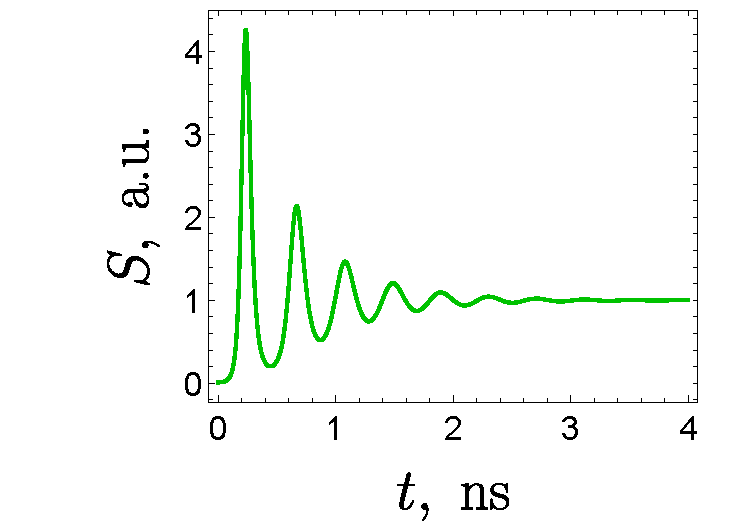
\includegraphics[width=\linewidth]{figures/laser_classic.pdf}
    \end{figure}
    
    \end{column}
    \begin{column}{.6\linewidth}
      Laser equations:
      \begin{align*}
        \frac{d S}{d t}&=-\gamma_{c} S+\Gamma g S \\
        \frac{d N}{d t}&=\frac{J}{e d}\left[1+\frac{\xi S(t-\tau)}{S_{0}}\right]-\gamma_{s} N-g S
      \end{align*}
    \end{column}
  \end{columns}

  Systems parameters:
  \begin{itemize}
    \iitem{ $f_r$ -- laser relaxation frequency. For our laser: \\
   \phantom{42} \hfill $f_r = 1.4 \div 3.2 \ \text{GHz}$.}
    \iitem{ $\tau$ -- delay time. $\tau \sim f_r^{-1} \sim 1 \text{ns}$.}
    \iitem{ $\xi = 0.1$ feedback parameter.}
  \end{itemize}
  
  % Here dimensionless variable $s = \dfrac{S}{S_0}$.  
\end{frame}

\begin{frame}
  \frametitle{Chaos parameters.}
  
  % Unimodular, multimodular and chaotic regimes of laser work:
  \begin{columns}
    \begin{column}{.4\linewidth}
      \begin{figure}
        \centering
        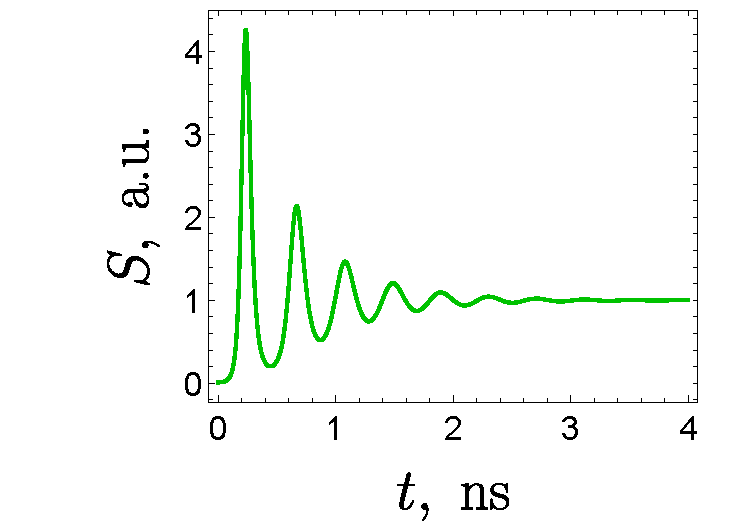
\includegraphics[width=\linewidth]{figures/laser_classic.pdf}
%        \caption{unbiased laser}
      \end{figure}
      \begin{figure}
        \centering
        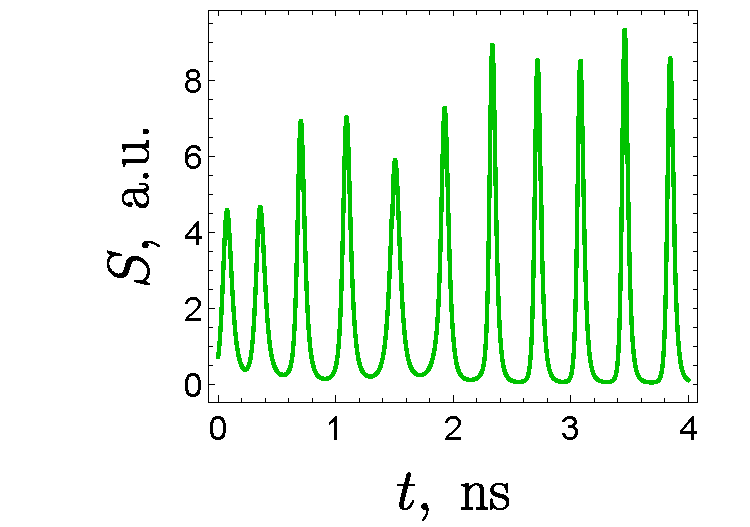
\includegraphics[width=\linewidth]{figures/laser_chaos.pdf}
      \end{figure}
      % another figure may be added with chaotic laser
    \end{column}
    \begin{column}{.6\linewidth}
      Chaos features:
      \begin{itemize}
        \iitem{ Unperiodic behaviour }
        \iitem{ Frequency doubling scenario $f \ \to \ 2 f \to \ 4f \to \dots \to \infty f$}
      \end{itemize}
      
      Chaos characteristics:
      \begin{itemize}
        \iitem{$\lambda $ -- (Lyapunov's exponent). Exponential divergence on time for close i.c.: $\Delta S (t) \approx  \Delta S (0) e^{\lambda t} $, where  $\Delta S (0) \ll S_0$.}
        \iitem{Embedded dimensions}
        \iitem{Shannon entropy}
      \end{itemize}
    \end{column}
  \end{columns}
  
  % Here dimensionless variable $s = \dfrac{S}{S_0}$.  
\end{frame}

\begin{frame}
  \frametitle{Chaos modelling. Different regimes.}
  
  % Unimodular, multimodular and chaotic regimes of laser work:
  \begin{figure}
    \centering
    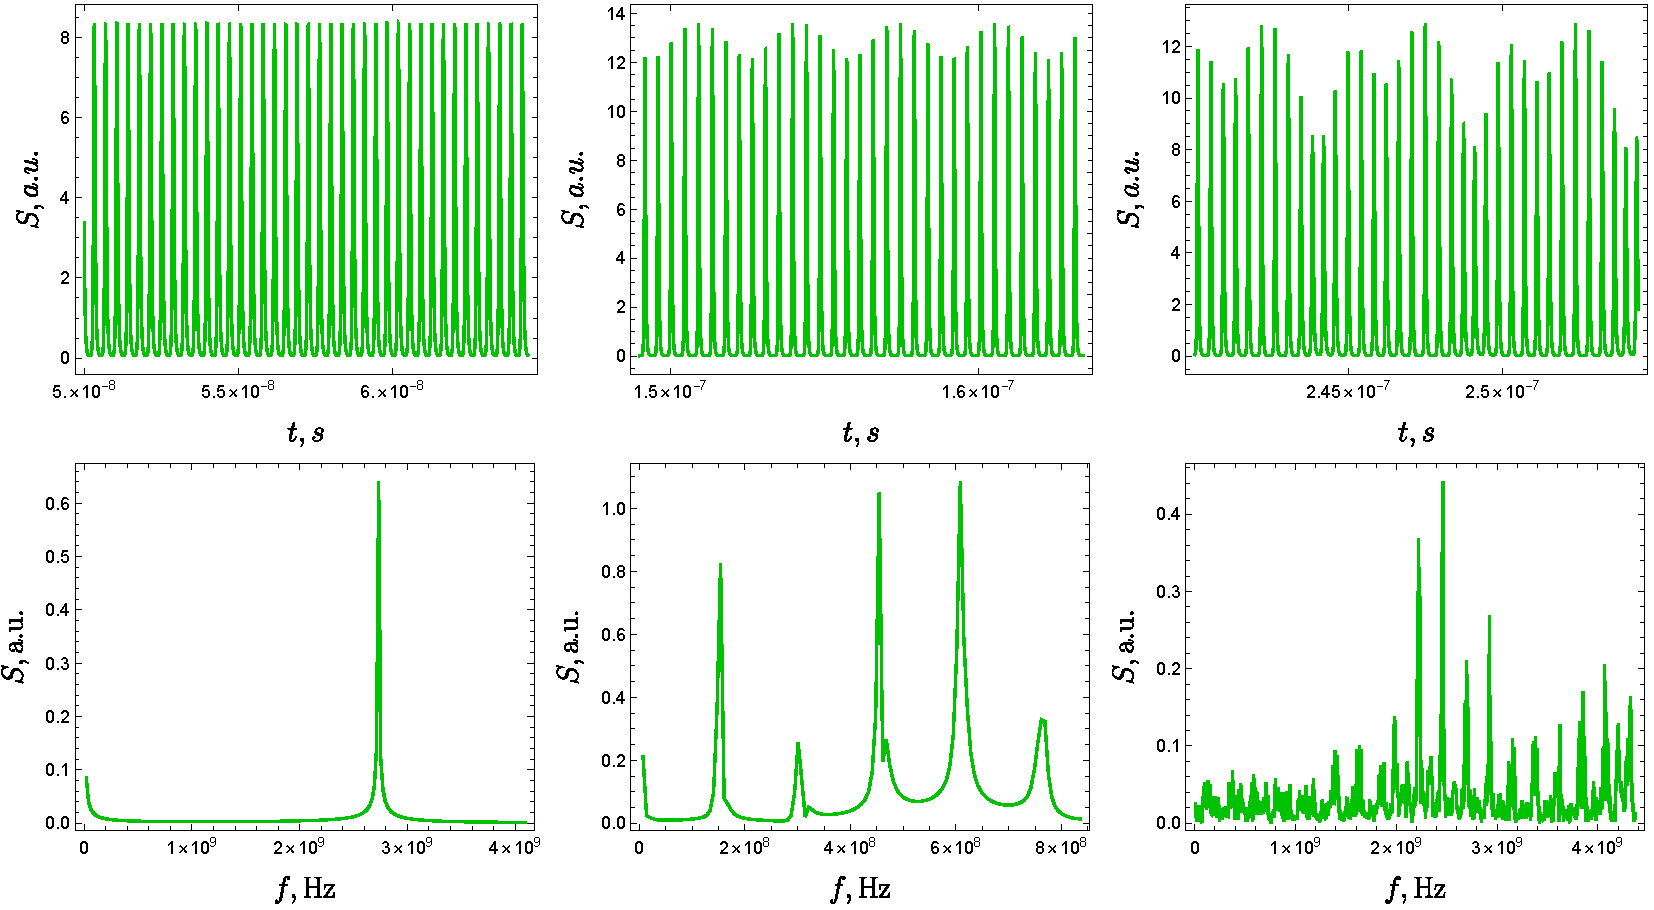
\includegraphics[width=\linewidth]{figures/chaos_and_spectra.pdf}
  \end{figure}
  
  \begin{center}
    \begin{tabular}{c|c|c}
      Delay time $\tau$:\ \ $2 \ T_r$ & $7.5 \ T_r$ & $12 \ T_r$
    \end{tabular}
  \end{center}
  
  % Here dimensionless variable $s = \dfrac{S}{S_0}$.
  
  
\end{frame}

\begin{frame}
  \frametitle{Chaos modelling.}
  Lyapunov exponents calculation for different points:
  
  $$\Delta S \sim \exp(\lambda t) \ \Rightarrow \ \log \Delta S = \lambda t + \const$$\\[5pt]
  
  \begin{figure}[h]
    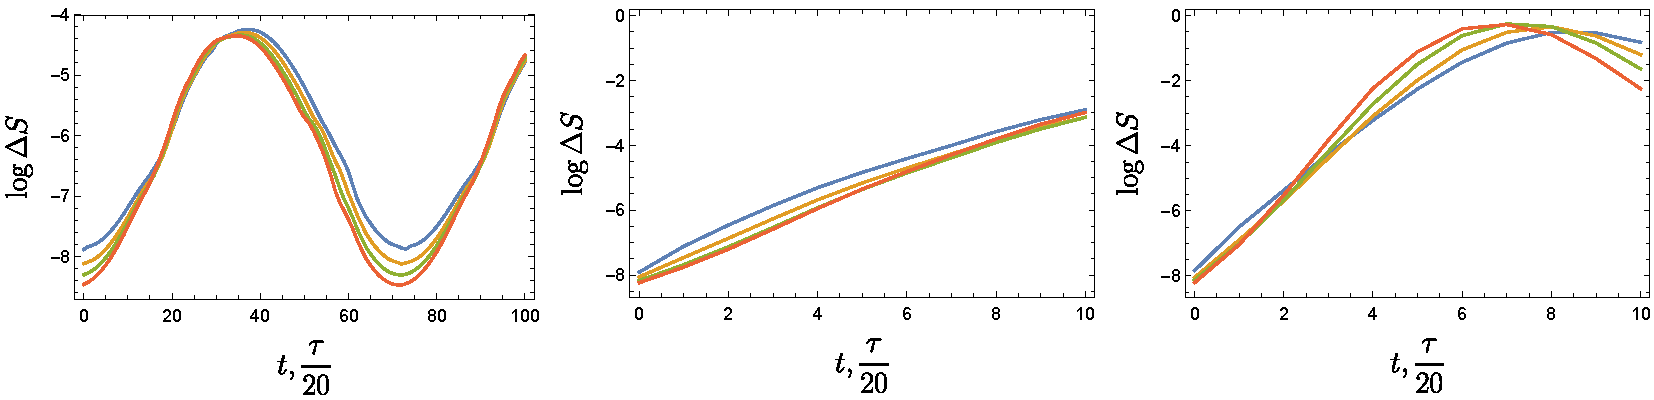
\includegraphics[width=1.0\textwidth]{figures/lyapunovs.pdf}
  \end{figure}
  
  \begin{center}
      \begin{tabular}{c|c|c|c}
        $\tau$ & $2 \ T_r$ & $7.5 \ T_r$ & $12 \ T_r$ \\ \hline
        $\lambda$ & $0.0$ & $1.62 \ f_r$ & $1.84 \ f_r$
      \end{tabular}
  \end{center}
    
  \phantom{42}
  
  \textbf{Chaos is possible!}. \\
  Thus, length of the fiber from the numerical analysis. $L \sim 1 \ \text{m}$
  
\end{frame}